\documentclass[]{article}
\usepackage[top=1in, bottom=1.25in, left=1.25in, right=1.25in]{geometry}
\usepackage{hyperref}
\usepackage{amsfonts}
\usepackage{amsmath}
\usepackage{graphicx}
\usepackage{float}

\title{\textbf{Linear models}}
\author{Yacine Debbabi}

\begin{document}

\maketitle

\tableofcontents

\noindent TOPICS TO COMPLETE: QR decomposition / GramSchmidt, F statistic, subgradient for XtX=I LASSO estimate, autocorrelations

\section{Model and OLS estimators}

The linear regression model has the form
\begin{equation}
y = \beta_0 + \sum_{j=1}^p \beta_j x_j + \epsilon
\end{equation}
where $\epsilon$ represents an unspecified error term. Given a set of training data $(x_1,y_1)$, ..., $(x_n,y_n)$, we can now estimate the parameter $\beta$. We form a design matrix $X=(1_n,X_1,...,X_p)$ where $X_j\in R^n$ for $j=1,...,p$, and an outcome vector $y\in R^n$. The least square estimation method consists of minimizing the residual sum of squares
\begin{eqnarray}
\mathrm{RSS(\beta)}&=&\sum_{i=1}^n \left(y_i-\left(\beta_0 + \sum_{j=1}^p \beta_j x_{ij}\right)\right)^2\\
&=&||Y-X\beta ||_2^2.
\end{eqnarray}
A unique solution $\hat{\beta}$ can be obtained by differentiating RSS with respect to the $\beta_j$'s,
\begin{equation}
\hat{\beta}=(X^TX)^{-1}X^Ty.
\end{equation}
\noindent Note that the above requires full rank for $X$, so that $X^TX$ is invertible. This is not the case when the columns of $X$ are not linearly independent. That would occur if two of the inputs were perfectly correlated, e.g. $X_2=3X_1$. In that case, there are (possibly distinct) solutions $\hat{\beta}$'s, although the fitted values $\hat{y}=X\hat{\beta}$ remain identical. Such rank deficiencies can also occur where the number of inputs $p$ exceeds the number of observations $n$. \\ \\
\noindent Up to now we have made minimal assumptions about the true distribution of the data. Assuming that (1) the observations $(x_i)_{i=1}^n$ are non-random and, (2) the errors are uncorrelated and have zero mean / constant variance $\sigma^2$, we can compute the variance of the OLS estimator as

\begin{equation}
\mathrm{Var}(\hat{\beta})=\sigma^2 (X^TX)^{-1}.
\end{equation}

\noindent To further pin down sampling properties for $\hat{\beta}$, we assume that the error is a Gaussian random variable, i.e. $E=(\epsilon_1, ..., \epsilon_n)\sim N(0,\sigma^2 I_n)$. This is a useful but also reasonable assumption in the light of the central limit theorem, if we were to decompose that noise into the addition of independent and identically distributed noises. That distributional assumption implies that $\hat{\beta}\sim N\left(\beta,\sigma^2(X^TX)^{-1}\right)$, and we can construct an estimator for the standard error $\sigma$ as
\begin{equation}
\hat{\sigma}^2:=\frac{1}{n-(p+1)}\sum_{i=1}^n (y_i-\hat{y}_i)^2
\end{equation}
where $\hat{Y}=X\hat{\beta}$. Using Cochran's theorem, we can show that $\hat{\beta}$ and $\hat{\sigma}^2$ are independent, and that $\hat{\sigma}^2 \sim \sigma^2 \chi_{n-p-1} /(n-p-1)$.  \\ 

\noindent These distributional properties allow to form tests of hypothesis and confidence intervals for $\beta$. To test the hypothesis that a particular coefficient $\beta_j$ is null, we form the Z-score
\begin{equation}
z_j = \frac{\hat{\beta}_j}{\hat{\sigma}\sqrt{(X^TX)^{-1}_{jj}}}.
\end{equation}
Under $H_0$: $\beta_j=0$, the Z-score follows a student distribution, i.e. $z_j\sim t_{n-p-1}$. We reject $H_0$ for large Z-score absolute values. Note that tail probabilities $\mathbb{P}(|t_n|>z)\approx\mathbb{P}(|N(0,1)|>z)$ for $n \to \infty$ and $z>2$, so the normal quantiles are typically used instead. The important orders of magnitude to remember are $\mathbb{P}(|N(0,1)|>2)\approx 5\%$ and $\mathbb{P}(|N(0,1)|>3)\approx 1\%$. We can also derive $1-2\alpha$ confidence intervals for $\beta_j$ as
\begin{equation}
\left(\beta_j-z^{1-\alpha}\hat{\sigma}\sqrt{(X^TX)^{-1}_{jj}}, \beta_j+z^{1-\alpha}\hat{\sigma}\sqrt{(X^TX)^{-1}_{jj}}\right)
\end{equation}
where $z^{1-\alpha}$ is the $1-\alpha$ percentile of the normal distribution by noting that $\mathbb{P}(|z_j|>z_{1-\alpha})=1-2\alpha$. Discuss approximation. We can extend the reasoning to higher dimensions and derive domains of confidence. We note that $A(\hat{\beta}-\beta)\sim N(0, \sigma^2 A (X^TX)^{-1} A^T)$, and so find that $(X^TX)^{-1/2}(\hat{\beta}-\beta)/\sigma\sim N(0, I_n)$ and $(\hat{\beta}-\beta)^T(X^TX)(\hat{\beta}-\beta)\sim\sigma^2 \chi^2_{p+1}$. We obtain a parameter-free law using $\hat{\sigma}^2$ as $(\hat{\beta}-\beta)^T(X^TX)(\hat{\beta}-\beta)/\hat{\sigma}^2\sim \chi^2_{p+1}/(\chi^2_{n-p-1}/(n-p-1))$. Noting that $\chi^2_{n-p-1}/(n-p-1)\rightarrow 1$, we obtain an approximate $1-2\alpha$ confidence interval as the set of $\beta$ 's such that
\begin{equation}
(\hat{\beta}-\beta)^T(X^TX)(\hat{\beta}-\beta)/\hat{\sigma}^2 \leq z_{\chi^2_{p+1}}^{1-\alpha}
\end{equation}
where $z_{\chi^2_{p+1}}^{1-\alpha}$ is the $1-\alpha$ quantile of the $\chi^2_{p+1}$ distribution. \\ \\
\noindent The Gaussian error assumption above allows us to derive a maximum likelihood estimator. The response $y$ is a Gaussian random vector so $Y\sim N(X\beta,\sigma^2I_n)$, so the likelihood can be written as
\begin{eqnarray}
L(\beta, \sigma):=\prod_{i=1}^n \frac{1}{\sigma\sqrt{2\pi}}\mathrm{exp} \left[-\frac{\left(y_i-(X\beta)_i\right)^2}{2\sigma^2}\right].
\end{eqnarray}
By maximizing the log-likelihood, one can also derive MLE estimators and find that $\hat{\beta}_{\mathrm{MLE}}=\hat{\beta}_{\mathrm{OLS}}$ and $\hat{\sigma}^2_{\mathrm{MLE}}=\hat{\sigma}^2\cdot(n-p-1)/n$. The error MLE is indeed biased.

\section{Optimality of OLS}

\noindent We first decompose the expected prediction error in general regression into several error sources, and then discuss the optimality of OLS estimates for linear regression functions. Consider the prediction of a response $y$ from an input $x$, i.e.
\begin{equation}
y = f(x)+\epsilon
\end{equation}
where $\epsilon$ is an unspecified error term independent from the input data. From a training set, we estimate a regression function $\hat{f}$ and make a prediction $\hat{f}(x)$ from input $x$. The expected prediction error can be written and decomposed as

\begin{eqnarray}
\mathbb{E}\left[\left(y-\hat{f}(x)\right)^2\right] &=& \mathbb{E}(\epsilon^2)+\mathbb{E}\left[\left(\hat{f}(x)-f(x)\right)^2\right] \\
&=&\mathbb{E}(\epsilon^2)+\mathrm{Var}\left(\hat{f}(x)\right)+\left(\mathbb{E}(\hat{f}(x))-f(x)\right)^2
\end{eqnarray}

\noindent This shows that - besides the irreducible model error - the estimator performance is controlled by its variance and its bias. This decomposition motivates the Gauss-Markov theorem, to show that the OLS estimator is the BLUE (best linear unbiased estimator) for linear regression problems, i.e. $f(x)=\beta^T x$. This also shows that beating the OLS performance requires trading away some bias against a reduction in variance.

\paragraph{Gauss-Markov theorem.} The least square estimate of parameter $a^T\beta$, i.e. $\hat{a}=a^T (X^TX)^{-1}X^Ty$, has a variance no larger than that of any linear unbiased estimate of $a^T\beta$.
\paragraph{Proof.} Let $Cy$ be a linear unbiased estimator of $a^T \beta$. We define $U=a^T(X^TX)^{-1}X^T$ and $D$ such that $C=U+D$. 
\begin{eqnarray}
\mathrm{Var}(Cy)&=&\sigma^2 C C^T\\
&=&\sigma^2 (UU^T+UD^T+DU^T+DD^T)\\
&=&\sigma^2 (a^T(X^TX)^{-1} a + DD^T+a^T(X^TX)^{-1}X^TD^T+DX(X^TX)^{-1}a)\\
&=&\sigma^2 (a^T(X^TX)^{-1} a + DD^T)\\
&\geq&\mathrm{Var}(\hat{a})
\end{eqnarray}
The simplification comes from the bias assumption: given $\mathbb{E}(Cy)=CX\beta=a^T\beta$ for all $\beta$, we have $CX=a^T$. This yields $DX=0$.

\section{Univariate regression}

The OLS solution is given by
\begin{eqnarray}
\hat{\beta}_0 &=& \bar{y}-\hat{\beta}_1\bar{x} \\
\hat{\beta}_1 &=& \frac{\langle x-\bar{x}, y-\bar{y} \rangle}{\langle x-\bar{x}, x-\bar{x} \rangle} = \hat{\rho}_{xy}\frac{\hat{\sigma}_y}{\hat{\sigma}_x}\\
\end{eqnarray}

\section{Regression with correlated predictors}

When the predictors are orthogonal, i.e. $\langle X_i,X_j\rangle=0$ if $i \neq j$, and both the predictors and response are mean centered, the OLS estimates (in absence of intercept) are then given by
\begin{equation}
\hat{\beta}_i=\frac{\langle X_i,y \rangle}{\langle X_i,X_i\rangle}.
\end{equation}
This shows that orthogonal inputs have no effect on each other's parameter estimates in the linear model. \\

\noindent Let us now analyse the impact of correlation between the predictors on regression coefficients. We can show that the estimate $\hat{\beta}_i$ is the contribution of $X_i$ once it has been adjusted for the remaining predictors, i.e. once we removed from $X_i$ the closest linear combination made from the remaining predictors. \\ \\
\noindent To see this, we build an orthogonal basis of Im(X), denoted $(z_i)_{i=0}^p$, following the Gram-Schmidt successive orthogonalization procedure; see appendix for more details. The coefficient associated with $z_p$ when regressing $y$ against $z_1,...,z_p$ is $\hat{\beta}_p=\langle z_p,y \rangle / \langle z_p,z_p \rangle$. Its variance is given by $\mathrm{Var}(\hat{\beta}_p)=\sigma^2/||z_p||^2$. \\ \\
\noindent Given that the residual $z_p$ is the only residual term containing $x_p$, $\hat{\beta}_p$ is also the OLS estimate for feature p. When feature $p$ shows little correlation with other features, $z_p$ is close to $X_p$, so the estimate matches the one found for uncorrelated inputs. When there exists a linear combination of features which approximate well feature $p$, the residual $z_p$ is small so the coefficient variance becomes large. This typically conduct to type II error, i.e. reject a relevant feature.

\section{Common data issues}

We discuss here common deviations from assumptions made in standard linear regression models. We discuss here how these deviations (a) modify estimator statistical properties (bias? variance change?), (b) affect feature selection via Z-scores, and (c) can be handled.

\subsection{Non-normality of residuals}

\paragraph{Consequences.} This breaks the assumption underpinning the hypothesis tests and confidence intervas derived. Asymptotic results however allow in certain cases to retain earlier results. To see this, consider a univariate regression model with no intercept. We can show that
\begin{equation}
\hat{\beta}-\beta=\frac{\sum_{i=1}^n x_i \epsilon_i}{\sum_{i=1}^n x_i^2}\xrightarrow{L}N\left(0, \sigma^2(X^TX)^{-1}\right)
\end{equation}
using a proof similar to the one used for the CLT.

\paragraph{Detection.} The normality of residuals is examined via the Q-Q plot. This reports the quantiles of the (normalized) residuals against the quantiles of a $N(0,1)$ distribution. Residuals are normalized for unit variance by dividing the residuals by their empirical standard deviation. The quantiles are computed by inverting their empirical cumulative distribution function, i.e. we compute $q_{\hat{F}_n}(u)=\hat{F}_n^{-1}(u)$ for a sequence of $u$'s spanning $[0,1]$.

\begin{figure}[H]
\center 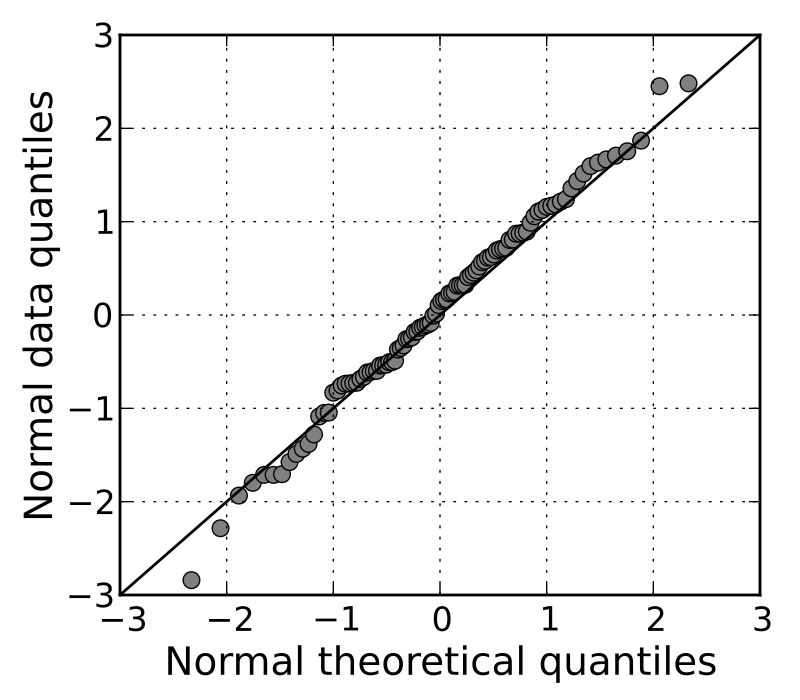
\includegraphics[scale=0.25]{qq_plot_example}
\caption{A normal Q–Q plot comparing randomly generated, independent standard normal data on the vertical axis to a standard normal population on the horizontal axis. The linearity of the points suggests that the data are normally distributed. Taken from \href{https://en.wikipedia.org/wiki/Q\%E2\%80\%93Q_plot}{Wikipedia}.}
\end{figure}

\subsection{Multicollinearity}

\paragraph{Consequences}

\begin{itemize}
\item Individual regression coefficients lose meaning. The usual interpretation of a regression coefficient is that it provides an estimate of the effect of a one unit change in an independent variable $X_1$ on the dependent variable $Y$. If $X_1$ is highly correlated with another variable $X_2$, changing $X_1$ only fails to capture the change in $X_2$ which the model would expect.
\item Standard errors of the affected coefficients tend to be large. This often leads to type II error, i.e. eliminate a relevant feature.
\item Small changes to the input data can lead to large changes in the model, even resulting in changes of sign of coefficient etimates.
\item This causes poor generalization if the pattern of collinearity in the new data differs that in the data that was fitted. To see this, the input data covers a restricted part of the parameter space in presence of multicollinearity, e.g. a line in a 2D space when we have two perfectly correlated features. Using the model outside this line means using the model outside of a region where it has been trained.
\end{itemize}

\paragraph{Detection}

\begin{itemize}
\item There are large changes in the estimated regression coefficients when a predictor variable is added or deleted.
\item A multivariate regression finds an insignificant coefficient for a particular explanator, yet a simple linear regression of the explained variable on this explanatory variable shows its coefficient to be significantly different from zero.
\item Use the variance inflation factor $\mathrm{VIF}_j:=1/(1-R_j^2)$, where $R_j^2$ is the coefficient of determination of a regression of feature $j$ on all the other features. A $\mathrm{VIF}$ above 5 or 10 usually indicates multicollinearity.
\item Use the condition number of the design matrix $X^TX$ with standardized predictors. This is computed as the square root of the maximum eigenvalue divided by its minimum eigenvalue. Values above 30 indicate multicollinearity.
\end{itemize}

\paragraph{How to handle this}

\begin{itemize}
\item Drop one of the variables. An explanatory variable may be dropped to produce a model with significant coefficients. However, you lose information (because you've dropped a variable). Omission of a relevant variable results in biased coefficient estimates for the remaining explanatory variables that are correlated with the dropped variable.
\item Ridge regression reduces the variance of coefficient estimates, which is introduced by the multicollinearity, by shrinking these coefficients to zero. This helps for instance when the presence of two highly correlated coefficients results in a widly large positive coefficient cancelling a similarly large negative coefficient on its correlated cousin.
\end{itemize}

\noindent More info can be found on \href{https://en.wikipedia.org/wiki/Multicollinearity}{Wikipedia}.

\subsection{Outliers}

Certain observations tend to have a significant impact on the model fit or statistics from which we derive conclusions. Their contribution is qualitatively captured by the quadratic term
\begin{equation}
(y_i-\hat{y}_i)^2
\end{equation}
present in the least square objective function. This can be significant either because the response $y_i$ or the prediction $\hat{y}_i$ (or equivalently, the feature inputs) are unusual. These observations can either be the product of error-prone measurements, in which case they should be clipped or removed, or provide essential information to the model.

\paragraph{Feature outliers.} These correspond to feature observations located in "unusual" regions of the feature space, and might cause "unusual" predictions. For instance, if $x_1$ and $x_2$ are highly correlated, a feature outlier would be present far away from their "usual line".  Feature outliers can be detected prior to model fit by computing the (robust) Mahalanobis distance of a single observation $x=(x_1,...,x_p)$ to the population mean $\mu$,
\begin{equation}
d(x,\mu):= (x-\mu)^T \Sigma^{-1} (x-\mu),
\end{equation}
where $\Sigma$ is the population covariance matrix. Assuming $x$ is sampled from a Gaussian distribution $N(\mu,\Sigma)$, we have sampling properties on the distance, i.e. $d(x,\mu)\sim\chi^2_p$. This allows us to identify outliers as observations with unlikely distances, i.e. $d(x,\mu)>q_{1-\alpha}$ where $q_{1-\alpha}$ is the $1-\alpha$ quantile associated with a $\chi^2_p$ distribution and $\alpha=0.05$ for instance. Note that outliers pollute the mean and covariance estimation. A robust distance can be obtained by using the Minimum Covariance Determinant estimator to estimate $\mu$ and $\Sigma$; see \href{https://scikit-learn.org/stable/auto_examples/covariance/plot_mahalanobis_distances.html#sphx-glr-auto-examples-covariance-plot-mahalanobis-distances-py}{here} for more details.\\

\noindent Some feature outliers can have a significant impact on coefficient estimates; we call these "high leverage points". This impact is quantified by the leverage statistics
\begin{equation}
h_{ii}=\frac{\partial \hat{y}_i}{\partial y_i}
\end{equation}
where $H=X(X^TX)^{-1}X^T$ is the "hat" projection matrix. To see this impact, consider a univariate regression model with centered input/response. The leverage statistics for observation $i$ is given by
\begin{equation}
h_{ii}=\frac{x_i^2}{n\hat{\sigma}_X^2}
\end{equation}
where $\hat{\sigma}_X^2$ is the empirical standard deviation for $X$. This shows the observation leverage increases with the distance to the sample mean.

\paragraph{Handling response/feature outliers.} The impact of outliers on model fit can be mitigated by changing the objective function. One can perform a weighted least square estimation where less weight is allocated to outliers, or by using alternative loss functions (e.g. Huber loss) to reduce the impact of large residuals on the fit.

\paragraph{Residual outliers.} Residual outliers are observations with unusually large absolute residuals $|r_i|=|y_i-\hat{y_i}|$. These do not necessarily have a significant impact on the fit, but will significantly increase the standard error estimation $\hat{\sigma}$. This might then suggest to eliminate a relevant feature (type 2 error). The residual abnormality can be quantified by the studentized residual
\begin{equation}
t_i = \frac{y_i-\hat{y_i}}{\hat{\sigma}\sqrt{1-h_{ii}}}\sim t_{n-p-1}.
\end{equation}
To prove the studentized distributional property, note that $Y-\hat{Y}=(I-H)Y$ where $H=X(X^TX)^{-1}X^T$ is the "hat" projection matrix, so $(y_i-\hat{y_i})/\sigma \sqrt{1-h_{ii}}\sim N(0,1)$. \\ \\
\noindent One can investigate their impact on conclusions we derive from various statistics by eliminating them from the fitting set.

\paragraph{Diagnostics tool.} Significant response/feature outliers and residual outliers can be rapidly observed from a studentized residuals / leverage diagram; see example below. Response/feature outliers can be identified as observations with leverage statistics that are more than 2-3 standard deviations away from the population mean. Residual outliers typically correspond to points with absolute studentized residuals greater than 2-3 and/or 

\begin{figure}[H]
\center 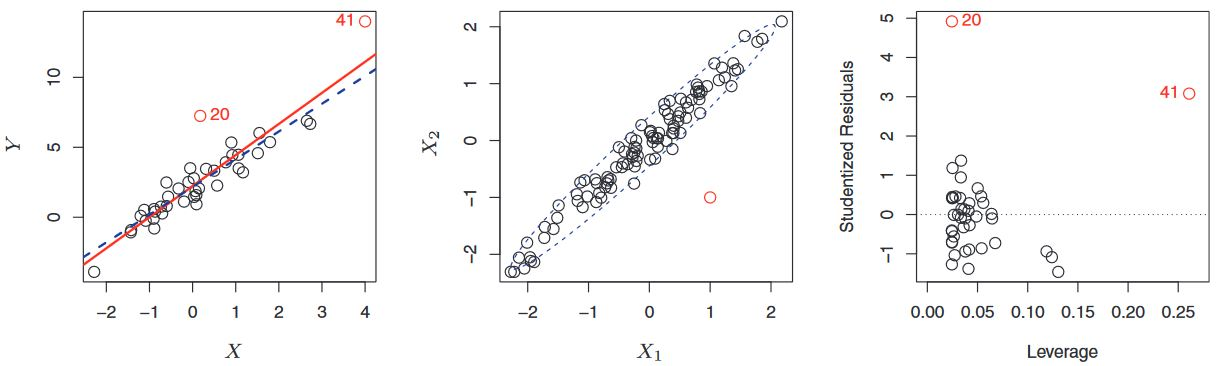
\includegraphics[scale=0.45]{outlier_examples.jpg}
\caption{(left) The $Y$ vs $X_1$ plot shows that observation 20 is a feature outlier while 41 is a high leverage point, (center) this 2D plot shows an example where the high leverage point would not be detectable from univariate plots, (right) diagnostic diagram.}
\end{figure}

\subsection{Heteroscedasticity}

This means that the standard deviation of the error term varies with the observation or input data.

\paragraph{Consequences} Heteroscedasticity does not bias the coefficient estimate, but implies the OLS is not the BLUE anymore - given this is a requirement of the Gauss Markov theorem. For a given error covariance matrix assumption, the generalized least square estimator is the BLUE. Heteroscedasticity implies hypothesis tests or Z-scores derived from a constant variance assumption are suspect.

\paragraph{How to handle this} 
\begin{itemize}
\item Transform the features or the outcome (by applying log for instance).
\item Use a weighted least square model with a specific covariance model to weight more accurately the observations.
\end{itemize}

\subsection{Autocorrelation of residuals}

To analyse the impact of residuals autocorrelation, we assume $\mathrm{Var}(\epsilon)=\Omega$, where $\Omega$ is different than $\sigma^2 I$ - as in the OLS estimation. The variance of the OLS coefficient can be written as $\mathrm{Var}(\hat{\beta})=(X^TX)^{-1}X^T \Omega X (X^TX)^{-1}$. We can examine that variance term for a univariate regression with unit-variance error and constant error covariance $\rho$ - so $\Omega$ is a matrix with 1's on the diagonal and $\rho$'s elsewhere. The coefficient variance can be written - up to a factor - as
\begin{eqnarray}
\mathrm{Var}(\hat{\beta}) &\propto& \sum_{i=1}^n x_i^2 + \rho \sum_{i\neq j} x_i x_j \\
&=& \sum_{i=1}^n x_i^2 - \rho \cdot n \cdot \hat{\sigma}_X^2
\end{eqnarray}

ABOVE SHOULD BE UPDATED WITH \href{http://web.sgh.waw.pl/~atoroj/econometric_methods/lecture_2_3_sc.pdf}{this}

\paragraph{Consequences}

\begin{itemize}
\item The OLS coefficient estimation remains unbiased, i.e. $E(\hat{\beta})=\beta_0$, but is no longer the minimum variance estimate.
\item With positive serial correlation ($\rho>0$), standard errors are underestimated, so Z-scores might indicate feature significance when there is none (type II error).
\end{itemize}



\section{Shrinkage}

\subsection{Ridge}

The Ridge estimate minimizes the penalized residual sum of squares,
\begin{eqnarray}
\hat{\beta}^{\mathrm{Ridge}} = \mathrm{argmin}_{\beta}\sum_{i=1}^n \left(y_i-(\beta_0 + \sum_{j=1}^p \beta_j x_{ij})\right)^2+\lambda \sum_{j=1}^p \beta_j^2
\end{eqnarray}
where the parameter $\lambda\geq 0$ controls the amount of shrinkage. Note that the intercept is not penalized. This optimization problem is equivalent to the standard least square optimization problem under the additional constraint that $\sum_{j=1}^p \beta_j^2 \leq t(\lambda)$. The solution is given by
\begin{equation}
\hat{\beta}^{\mathrm{Ridge}}=(X^TX+\lambda I)^{-1}X^Ty.
\end{equation}
Note that the solution is not equivariant under scaling of the inputs, so one normally standardizes the input - by replacing $X_i$ by $(X_i-\bar{X}_i)/\sigma_{X_i}$ - before computing the Ridge estimate. \\ \\
Ridge makes sure a unique solution exists regardless of the correlation structure between features, i.e. $X^TX+\lambda I$ is invertible regardless of $X$. We can compute the Ridge estimator variance as

\begin{equation}
\mathrm{Var}(\hat{\beta}^{\mathrm{Ridge}})= \sigma^2 (X^TX+\lambda I)^{-1}X^T X(X^TX+\lambda I)^{-1}
\end{equation}
and can verify in the orthonormal case ($X^TX=I$) that Ridge offers a reduced variance, i.e. $\mathrm{Var}(\hat{\beta}^{\mathrm{Ridge}})\leq \mathrm{Var}(\hat{\beta}^{\mathrm{OLS}})$.\\

\noindent What if we include an exact copy of the data in a univariate Ridge regression and refit? Let us denote $(\hat{\beta}_1,\hat{\beta}_2)$ the new Ridge solution. That solution must be such that $\hat{\beta}_1=\hat{\beta}_2$, so $\hat{\beta}_1^2+\hat{\beta}_2^2$ is minimal. Under that constraint the solution is obtained from the univariate Ridge estimate $\hat{\beta}$ as $\hat{\beta}_1=\hat{\beta}_2=\hat{\beta}/2$. \\ \\
When there are many correlated inputs, their coefficients can become poorly determined and exhibit high variance. A wildly large positive coefficient on one variable can be canceled by a similarly large negative coefficient on its correlated cousin. Ridge alleviates this problem by penalizing large coefficients, and therefore reduces variance.

\subsection{Lasso}

The Lasso estimate minimizes the penalized residual sum of squares
\begin{eqnarray}
\hat{\beta}^{\mathrm{Lasso}} = \mathrm{argmin}_{\beta}\sum_{i=1}^n \left(y_i-(\beta_0 + \sum_{j=1}^p \beta_j x_{ij})\right)^2+\lambda \sum_{j=1}^p |\beta_j|,
\end{eqnarray}
which is equivalent to the standard least square optimization problem under the additional constraint that $\sum_{j=1}^p |\beta_j| \leq t(\lambda)$. The solution is non linear in the $y_i$, and there is no closed form solution unless $X$ is orthonormal, i.e. $X^T X=I_n$. Then we have
\begin{equation}
\hat{\beta}^{\mathrm{Lasso}}_j = \mathrm{sign}(\hat{\beta}_j^{\mathrm{OLS}})(|\hat{\beta}_j^{\mathrm{OLS}}|-\lambda)_+.
\end{equation}
\noindent The Lasso can be computed via a simple coordinate descent. We start from the OLS estimate and optimize successively over each parameter. Say our current estimate is $(\beta_0^{m+1},...,\beta_{j-1}^{m+1},\beta_j^m,...,\beta_p^m)$. We can now estimate 
\begin{eqnarray}
\beta_{j}^{m+1} = \mathrm{argmin}_{\beta_j}\sum_{i=1}^n \left((y_i-\beta_0 - \sum_{k\neq j} \beta_k x_{ik})-\beta_j x_{ij}\right)^2+\lambda |\beta_j|
\end{eqnarray}
by applying the soft-thresholding operator above on the corrected response $Y-X_{-j}\beta_{-j}$. With orthonormal inputs, the OLS estimate for coefficient $j$ is not influenced by values taken by $\beta_{-j}$, so we iterate only once per feature.

\subsection{Shrinkage estimators as Bayesian estimates}


\section{Generalized least squares}

Generalized least squares (GLS) is a technique for estimating the unknown parameters in a linear regression model when there is a certain degree of correlation between the residuals in a regression model. \\ \\
The model assumes the conditional variance of the error term given $X$ is a known non-singular covariance matrix $\Omega$, i.e. $\mathrm{Cov}(\epsilon|X)=\sigma^2\Omega$. The standard least square model is the particular case of $\Omega=I_n$. Under that model assumption, we note that the transformed data $X^*=C^T X$ and $y^*=C^T y$, where $\Omega=C C^T$ is the Cholesky decomposition of $\Omega$, follows the standard model. This means the BLUE coefficient estimator is given by $\hat{\beta}^*=((X^*)^TX^*)^{-1}(X^*)^Ty^*$. This yields the GLS estimator
\begin{equation}
\hat{\beta}_{\mathrm{GLS}}=(X^T\Omega^{-1}X)^{-1}X^T\Omega^{-1}y.
\end{equation}

\noindent Resource can be found \href{http://web.vu.lt/mif/a.buteikis/wp-content/uploads/PE_Book/4-7-Multiple-heteroskedastic.html}{here}.\\

(GLS is equivalent to the OLS with unit standard error when applying a linear transformation $\Omega^{-1/2}$ to the data. \\ \\
A special case of GLS called weighted least squares (WLS) occurs when all the off-diagonal entries of $\Omega$ are 0. This situation arises when the variances of the observed values are unequal (i.e. heteroscedasticity is present), but where no correlations exist among the observed variances.

\noindent To see this, consider a univariate model $Y=\beta X$. Say we have 2 observations with standard errors $\sigma_1$ and $\sigma_2$, and $\sigma_1\gg\sigma_2$. The log loss function can be written as $L(\beta) = (y_1-\beta\cdot x_1)/ \sigma_1^2+(y_2-\beta\cdot x_2)/ \sigma_2^2$. The coefficient estimate is approximately equal to $\hat{\beta}_H=y_1/x_1$. The OLS coefficient estimate ignores $\sigma$'s and is given by $\hat{\beta}_{OLS}=(x_1\cdot y_1+x_2\cdot y_2)/ (x_1^2+x_2^2)$. Denote by $\beta_0$ the true regression coefficients; both estimates are unbiased, i.e. $E(\hat{\beta}_H)=E(\hat{\beta}_{OLS})=\beta_0$. However they have different variances, i.e. $\mathrm{Var}(\hat{\beta}_H)=\sigma_1^2/x_1^2$ and $\mathrm{Var}(\hat{\beta}_{OLS})=(x_1^2\sigma_1^2+x_2^2\sigma_2^2)/ (x_1^2+x_2^2)^2$.


\section{Appendix}

\subsection{Standard laws}

\begin{itemize}
\item Let $X_1$, ..., $X_p$ be i.i.d. RVs such that $X_i\sim N(0,1)$, then $\sum_{i=1}^p X_i^2 \sim \chi^2_p$.
\item Let $U$, $V$ be two RVs such that $U\sim N(0,1)\perp \!\!\! \perp V\sim \chi^2_p$, then $U/ \sqrt{V/p}\sim t_p$.
\item Let $U$, $V$ be two RVs such that $U\sim \chi^2_p\perp \!\!\! \perp V\sim \chi^2_q$, then $(U/p)/ (V/q)\sim F_{p,q}$.
\end{itemize}

\subsection{Central limit theorem}

\paragraph{Theorem.} Let $(X_i)_{i=1}^n$ be a sequence of i.i.d. RVs with $\mathbb{E}(X)=\mu$ and $\mathrm{Var}(X)=\sigma^2<\infty$. Then
\begin{equation}
\frac{\sqrt{n}(\bar{X}_n-\mu)}{\sigma}\xrightarrow{d}N(0,1).
\end{equation}

\paragraph{Proof.} The result can be proved using characteristic functions as follows. For any $u\in R$,
\begin{eqnarray}
\mathbb{E}\left[\exp\left(iu\frac{\sqrt{n}(\bar{X}_n-\mu)}{\sigma}\right)\right] &=& \mathbb{E}\left[\exp\left(iu\frac{\sum_{i=1}^n X_i-\mu}{\sigma\sqrt{n}}\right)\right] \\
&=& \prod_{i=1}^n \mathbb{E}\left[\exp\left(i\frac{u}{\sqrt{n}}\frac{X_i-\mu}{\sigma}\right)\right] \\
&=& \mathbb{E}\left[\exp\left(i\frac{u}{\sqrt{n}}\frac{X_-\mu}{\sigma}\right)\right]^n
\end{eqnarray}
Let us denote $f$ the characteristic function of $Y:=(X-\mu)/\sigma$, i.e. $f(u)=\mathbb{E}\left[e^{iuY}\right]$. Given we have $f'(u)=\mathbb{E}\left[iYe^{iuY}\right]$ and $f''(u)=-\mathbb{E}\left[Y^2e^{iuY}\right]$, we can approximate the above as

\begin{eqnarray}
\mathbb{E}\left[\exp\left(iu\frac{\sqrt{n}(\bar{X}_n-\mu)}{\sigma}\right)\right]^n &\approx& \left(1+\frac{u}{\sqrt{n}}f'(0)+\frac{1}{2}\frac{u^2}{n}f''(0)\right)^n \\
&=& \left(1-\frac{u^2}{2n}\right)^n\xrightarrow{n \to \infty}e^{-u^2/2},
\end{eqnarray}
and therefore find that the initial characteristic function converges to those of a $N(0,1)$ RV.

\subsection{Type I / II error}

Type I error (false positive / an innocent is convicted) is the rejection of a true $H_0$. Type II error (false negative / a guilty person is freed) is the non-rejection of a false $H_0$.

\subsection{Cochran's theorem}

\paragraph{Theorem.} Let $Y\sim N(\mu, \sigma^2 I_n)$. Let $E_1$, ..., $E_p$ be a finite sequence of orthogonal vector subspaces of $R^n$ such that $\sum_{j=1}^p \mathrm{dim}(E_j) = n$. We denote by $\Pi_j$ the \textbf{orthogonal} projection matrix on $E_j$. Then, we have that (a) $\Pi_1 Y$, ..., $\Pi_p Y$ are independent, and (b) $\Pi_j Y \sim N(\Pi_j\mu, \sigma^2\Pi_j)$ and $||\Pi_j (Y-\mu)/\sigma||_2^2 \sim \chi^2(\mathrm{dim}(E_j))$ for $j=1,...,p$.

\paragraph{Notes.} A \textbf{projection} $P$ on a vector space $V$ is a linear operator $P: V \rightarrow V$ such that $P^2=P$. A projection matrix $P$ is a square matrix such that $P^2=P$. $P$ is called an \textbf{orthogonal projection matrix} if we additionally have $P=P^T$.

\paragraph{Proof.} We define $A=(\Pi_1,...,\Pi_p)^T\in R^{np \times n}$ - i.e. we stack the projection matrices along the diagonal - and note that $Z=AY\sim N(A\mu, \sigma^2 AA^T)$. Computing $AA^T$ reduces to computing $\Pi_j\Pi_k^T=\Pi_j\Pi_k=0$ if $j\neq k$ and $\Pi_j$ else. This is obtained from the symmetry of the orthogonal projection matrices, i.e. $\Pi_j^T=\Pi_j$, and the orthogonality of the underlying subspaces, i.e. $\mathrm{Im}(\Pi_k)\subset\mathrm{Ker}(\Pi_j)$.\\
We diagonalize the j-th orthogonal projection matrix as $\Pi_j=P_j^TD_jP_j$ where $D$ is a diagonal matrix with 1s on the first $\mathrm{dim}(E_j)$ elements of the diagonal and 0s elsewhere. After denoting $Z:=(Y-\mu)/\sigma$, we prove the last assertion by noting that
\begin{eqnarray}
||\Pi_j (Y-\mu)/\sigma||_2^2 &=& Z^T\Pi_j^T\Pi_j Z \\
&=& Z^T P_j^T D_j P_j Z \\
&=& \sum_{i=1}^{\mathrm{dim}(E_j)} (P_j Z)_i^2
\end{eqnarray}
and that $P_j Z$ is a Gaussian vector with independent components and $(P_j Z)_i \sim N(0,1)$ for $i\leq \mathrm{dim}(E_j)$.

\subsection{Gram-Schmidt orthogonalization}

COMPLETE SECTION

\end{document}
